\section{Analyse de la sensibilité des réseaux convolutifs}

Dans cette troisième et dernière partie, nous allons analyser la sensibilité des réseaux convolutifs à leur entrée sur une tâche de classification d’image de type ImageNet. L’objectif est de visualiser et de comprendre à quels pixels le réseau est sensible lors de la prise de décision de classification.

\subsection{Algorithmes de Class Activation Mapping (CAM)}

Les algorithmes de Class Activation Mapping (CAM) sont des techniques utilisées en vision par ordinateur pour visualiser les régions d'une image qui influencent le plus la décision d'un modèle de classification. Ces méthodes génèrent des cartes d'activation qui mettent en évidence les zones importantes de l'image pour une classe donnée.\\

Dans la page GitHub \href{https://github.com/utkuozbulak/pytorch-cnn-visualizations}{utkuozbulak/pytorch-cnn-visualizations}, différentes méthodes de Class Activation Mapping (CAM) sont présentées pour visualiser quelles régions d'une image influencent le plus la décision d'un modèle CNN :

\begin{itemize}
    \item \textbf{CAM} : Utilise une combinaison pondérée des activations de la dernière couche convolutionnelle pour générer une carte de chaleur des régions les plus influentes.
    \item \textbf{Grad-CAM} : Utilise les gradients de la classe cible par rapport aux cartes d'activation pour générer une carte de chaleur plus précise.
    \item \textbf{Grad-CAM++} : Améliore Grad-CAM en prenant en compte les contributions positives de chaque pixel avec des poids spécifiques.
    \item \textbf{Score-CAM} : Utilise les scores de prédiction pour évaluer l'importance des caractéristiques, évitant ainsi les coûts de calcul associés aux gradients.
\end{itemize}

\subsection{Activation d'une classe sur des images}

Nous allons maintenant nous intéresser à l'activation d'une classe sur différentes images. Notre étude utilisera trois images : 
\begin{itemize}
    \item Une image contenant un seul objet de la classe.
    \item Une image contenant plusieurs objets de la classe.
    \item Une image ne contenant aucun objet de la classe.
\end{itemize}

\subsubsection{Choix du setup}

Pour mener à bien cette étude, nous avons sélectionné un setup composé d'un modèle backbone, d'une méthode de CAM et d'une classe cible. Nos choix se sont portés sur : 
\begin{itemize}
    \item Le modèle \texttt{regnet\_y\_400mf}, qui offre un bon équilibre entre performance et efficacité.
    \item La méthode \textbf{Grad-CAM++}, car elle est l'une des méthodes les plus complètes tout en restant légère par rapport à Score-CAM.
    \item La classe à détecter sera \textit{tennis ball}.
\end{itemize}

\newpage

Voici les images utilisées pour l'étude :

\begin{table}[H]
    \centering
    \begin{tabular}{|c|c|c|}
      \hline
      \textbf{Un objet} & \textbf{Plusieurs objets} & \textbf{Aucun objet} \\
      \hline
      \includegraphics[width=0.3\textwidth]{tennis_ball.jpg} &
      \includegraphics[width=0.3\textwidth]{tennis_balls.jpg} &
      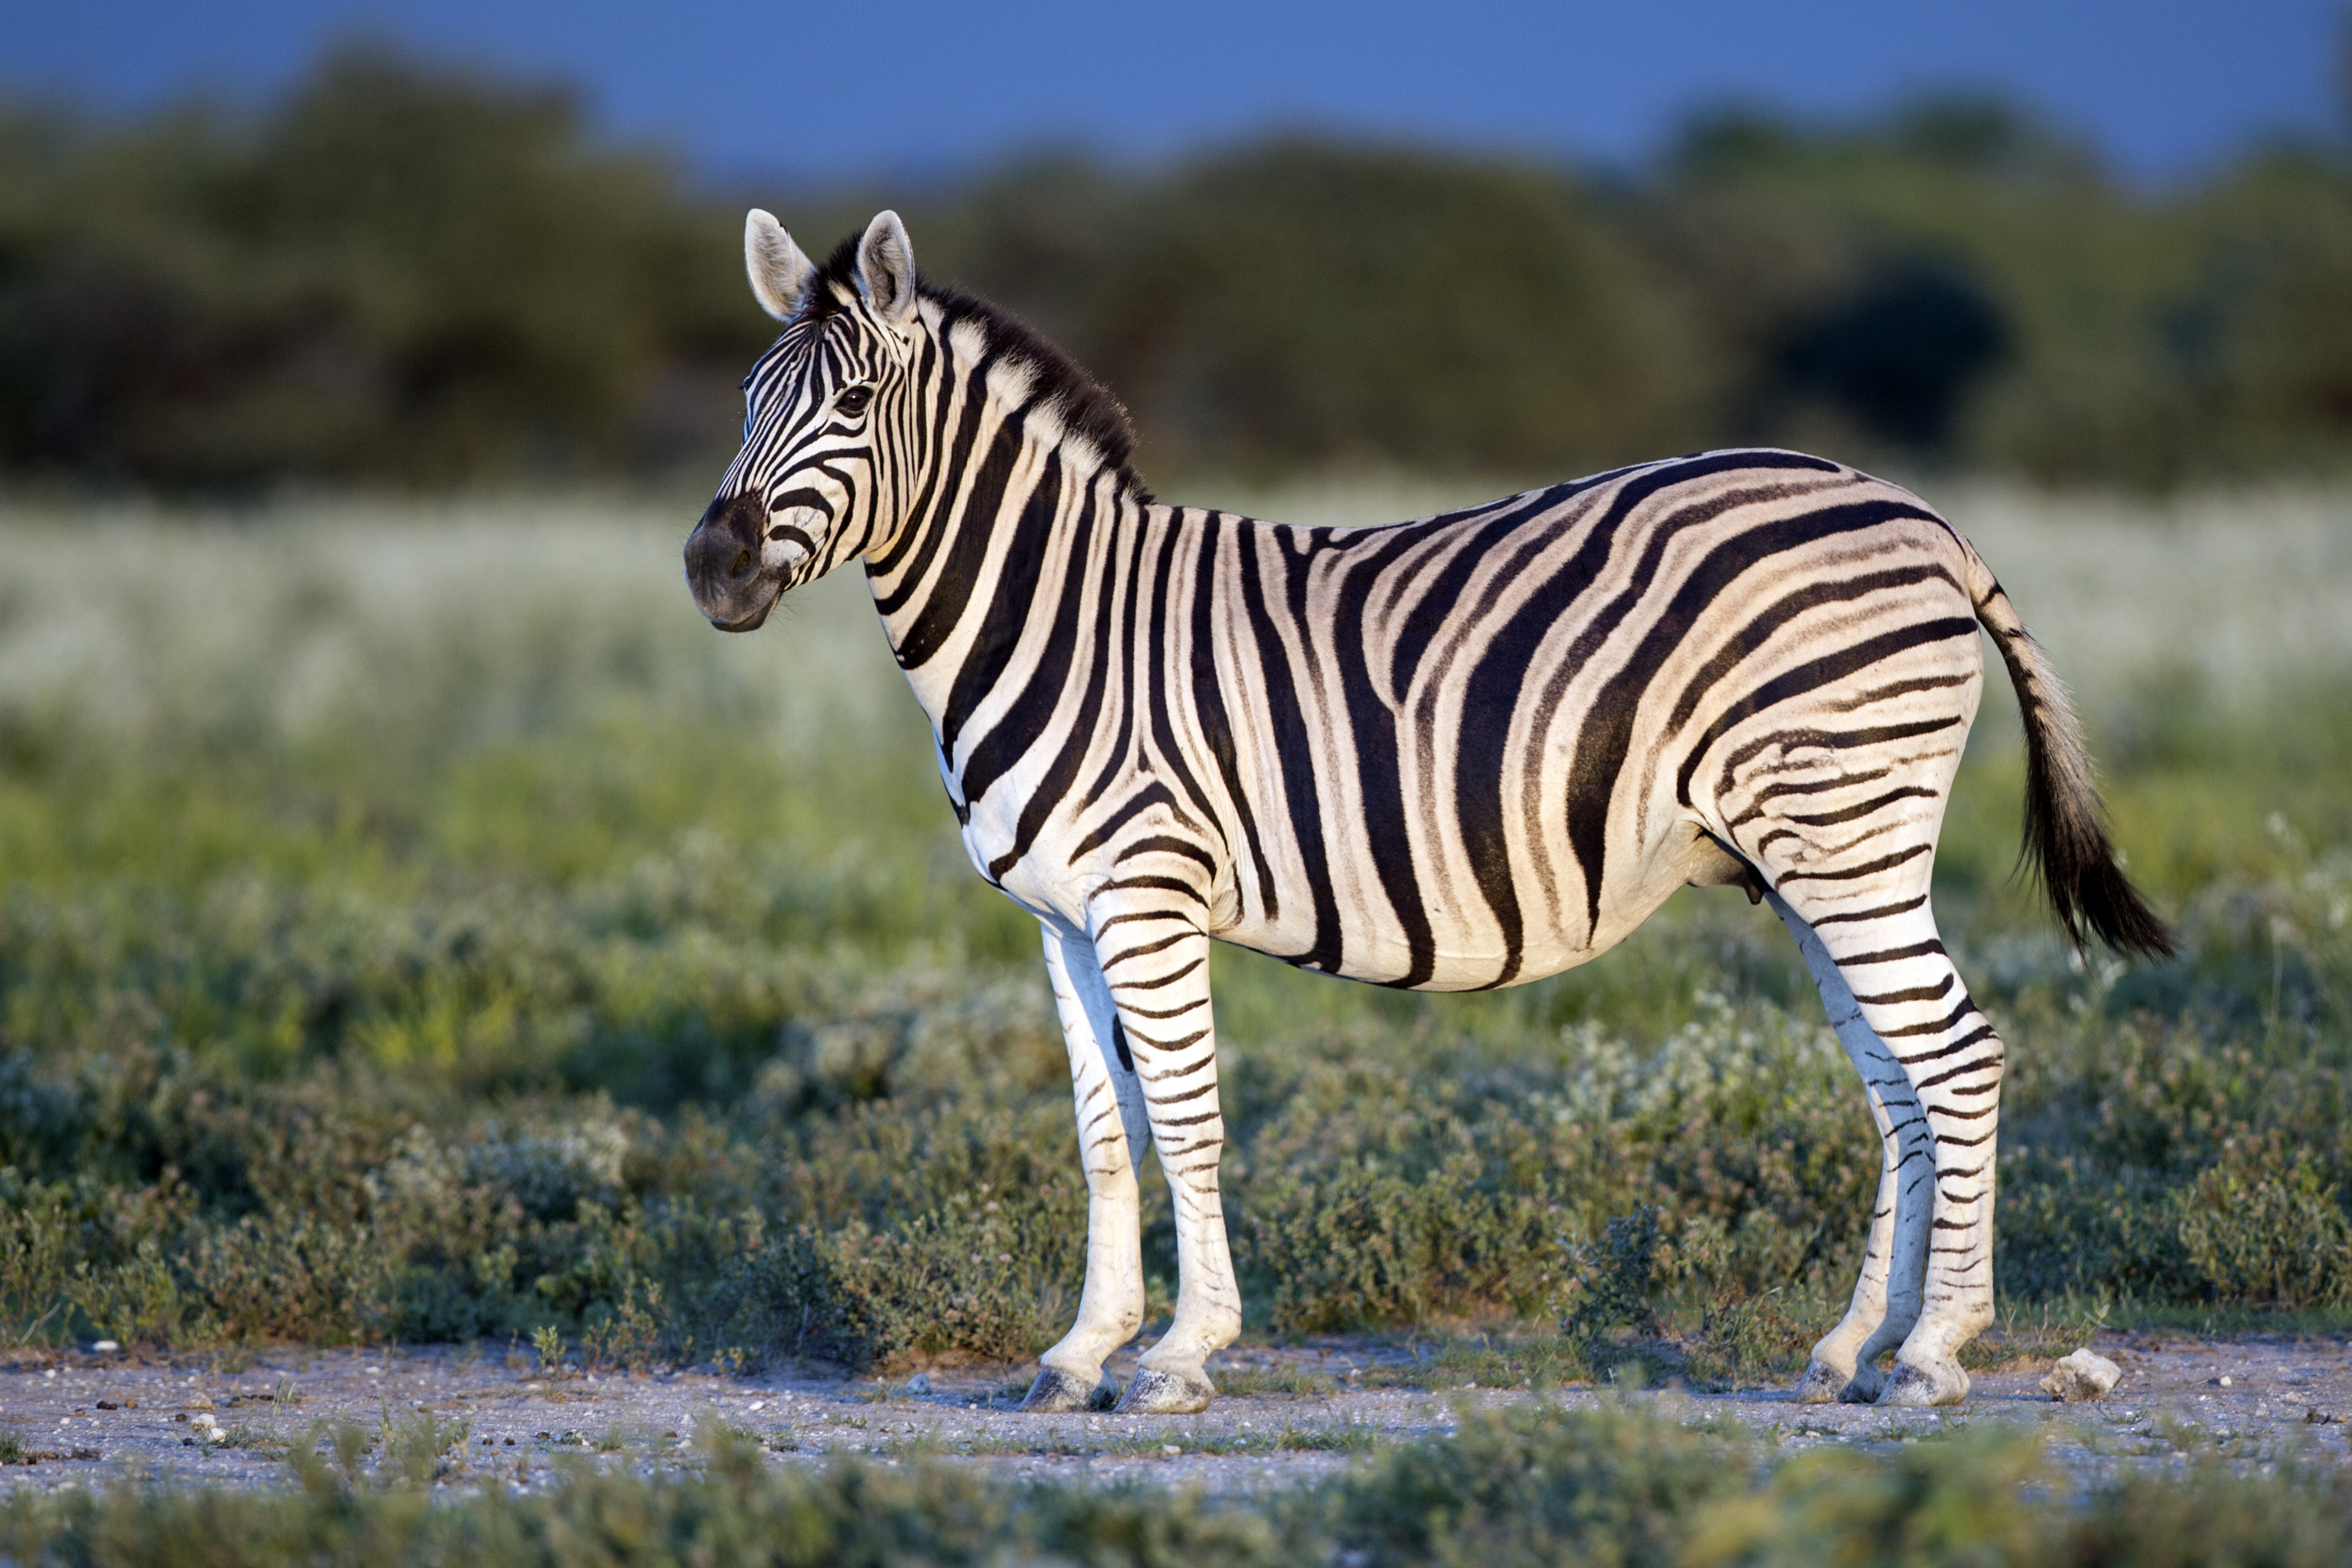
\includegraphics[width=0.3\textwidth]{z.jpg} \\
      \hline
    \end{tabular}
    \caption{Images utilisées pour l'analyse CAM.}
    \label{tab:images_cam}
\end{table}

\subsubsection{Analyse des résultats}
\begin{figure}[H]
    \centering
    \includegraphics[width=0.9\linewidth]{CAM_tennis_ball.png}
    \caption{Résultat de l'activation pour une balle de tennis seule.}
\end{figure}
Pour la balle de tennis seule, le modèle identifie l'objet avec un score de confiance de \textbf{99.92\%}. La carte thermique dans la partie "Overlayed CAM" montre clairement les zones qui contribuent le plus à la classification, avec la région la plus brillante (jaune/rouge) concentrée précisément sur la balle de tennis. La carte d'activation brute ("Raw CAM") révèle les pixels activés avant lissage, indiquant que le modèle se concentre principalement sur la forme circulaire et la couleur jaune-vert caractéristique de la balle.

\begin{figure}[H]
    \centering
    \includegraphics[width=0.9\linewidth]{CAM_tennis_balls.png}
    \caption{Résultat de l'activation pour plusieurs balles de tennis.}
\end{figure}
Pour l'image contenant plusieurs balles de tennis tenues dans une main, nous obtenons un score quasi-identique de \textbf{99.93\%}. Cela démontre la robustesse du modèle qui parvient à identifier correctement les balles de tennis même lorsqu'elles sont multiples et partiellement masquées. L'activation se concentre principalement sur les balles elles-mêmes plutôt que sur la main qui les tient, ce qui indique que le modèle a bien appris les caractéristiques distinctives des balles de tennis (texture, couleur, forme) et non le contexte environnant.

\begin{figure}[H]
    \centering
    \includegraphics[width=0.9\linewidth]{CAM_zebra.png}
    \caption{Résultat de l'activation pour l'image d'un zèbre.}
\end{figure}
Enfin, pour l'image contenant un zèbre, le modèle retourne un score de confiance de \textbf{0.00\%}, indiquant correctement l'absence de balle de tennis. Il est intéressant de noter que malgré ce score nul, la carte thermique montre tout de même certaines activations, notamment autour de la tête du zèbre et sur certaines parties de son corps. Ces activations pourraient s'expliquer par la recherche par le modèle de formes arrondies ou de couleurs qui présentent des similitudes partielles avec les caractéristiques des balles de tennis.

\newpage
\subsubsection{Transformation de l'image}

Afin d'analyser plus profondément les performances et la fiabilité de notre modèle de détection d'objets, nous avons réalisé une série de tests en appliquant deux types distincts de transformations d'image (modification de luminosité et changement de perspective) sur notre image de référence contenant une unique balle de tennis. Cette approche nous permet d'évaluer la robustesse du modèle dans des conditions variables.\\\\
Pour chaque type de transformation, nous avons généré une séquence de 10 images présentant une intensité croissante de modification, permettant ainsi d'observer l'évolution progressive des performances du modèle face à ces altérations.

\begin{table}[H]
    \centering
    \begin{tabular}{|c|c|c|c|}
      \hline
      \textbf{Image} & \textbf{Score} & \textbf{Image} & \textbf{Score} \\
      \hline
      \includegraphics[width=0.25\textwidth]{images/brightness_1.jpg} & \Large 92.3 &
      \includegraphics[width=0.25\textwidth]{images/brightness_2.jpg} & \Large 99.92 \\
      \hline
      \includegraphics[width=0.25\textwidth]{images/brightness_3.jpg} & \Large 99.23 &
      \includegraphics[width=0.25\textwidth]{images/brightness_4.jpg} & \Large 99.32 \\
      \hline
      \includegraphics[width=0.25\textwidth]{images/brightness_5.jpg} & \Large 99.49 &
      \includegraphics[width=0.25\textwidth]{images/brightness_6.jpg} & \Large 98.55 \\
      \hline
      \includegraphics[width=0.25\textwidth]{images/brightness_7.jpg} & \Large 92.11 &
      \includegraphics[width=0.25\textwidth]{images/brightness_8.jpg} & \Large 80.48 \\
      \hline
      \includegraphics[width=0.25\textwidth]{images/brightness_9.jpg} & \Large 75.13 &
      \includegraphics[width=0.25\textwidth]{images/brightness_10.jpg} & \Large 74.37 \\
      \hline
    \end{tabular}
    \caption{Comparaison des scores - luminosité}
    \label{tab:brightness_scores}
\end{table}

L'analyse des scores de confiance révèle plusieurs tendances significatives concernant la robustesse du modèle face aux variations de luminosité :

\begin{enumerate}
    \item Zone optimale de détection : Les scores les plus élevés ($>99\%$) sont obtenus pour les images avec une luminosité modérée (images 2 à 5), ce qui suggère une plage de fonctionnement optimal du modèle.
    \item Dégradation progressive : On observe une diminution notable des performances aux extrémités du spectre de luminosité :
    \begin{itemize}
        \item Pour les images très sombres (image 1), le score descend à 92.3\%
        \item Pour les images très lumineuses (images 7 à 10), on constate une dégradation encore plus marquée, avec des scores descendant jusqu'à 74.37\%
    \end{itemize}
    \item Seuil critique : La baisse significative des scores en dessous de 80\% pour les images fortement surexposées (images 9 et 10) indique un seuil critique au-delà duquel la fiabilité du modèle devient préoccupante.
\end{enumerate}

Cette tendance s'explique probablement par la perte de contraste et de détails caractéristiques de la balle de tennis dans les conditions extrêmes d'éclairage. Dans les images très lumineuses, la texture distinctive jaune-verte de la balle tend à se confondre avec l'arrière-plan en raison de la surexposition, tandis que dans les images très sombres, les contours et le contraste sont réduits.

\begin{table}[H]
    \centering
    \begin{tabular}{|c|c|c|c|}
      \hline
      \textbf{Image} & \textbf{Score} & \textbf{Image} & \textbf{Score} \\
      \hline
      \includegraphics[width=0.25\textwidth]{images/perspective_1.jpg} & \Large 99.92 &
      \includegraphics[width=0.25\textwidth]{images/perspective_2.jpg} & \Large 99.91 \\
      \hline
      \includegraphics[width=0.25\textwidth]{images/perspective_3.jpg} & \Large 99.94 &
      \includegraphics[width=0.25\textwidth]{images/perspective_4.jpg} & \Large 99.95 \\
      \hline
      \includegraphics[width=0.25\textwidth]{images/perspective_5.jpg} & \Large 99.94 &
      \includegraphics[width=0.25\textwidth]{images/perspective_6.jpg} & \Large 99.94 \\
      \hline
      \includegraphics[width=0.25\textwidth]{images/perspective_7.jpg} & \Large 0.54 &
      \includegraphics[width=0.25\textwidth]{images/perspective_8.jpg} & \Large 99.27 \\
      \hline
      \includegraphics[width=0.25\textwidth]{images/perspective_9.jpg} & \Large 99.47 &
      \includegraphics[width=0.25\textwidth]{images/perspective_10.jpg} & \Large 99.69 \\
      \hline
    \end{tabular}
    \caption{Comparaison des scores - perspective}
    \label{tab:perspective_scores}
\end{table}

L'analyse des scores de confiance pour les transformations de perspective révèle un comportement nettement différent de celui observé pour les variations de luminosité : 

\begin{enumerate}
    \item Haute robustesse générale : Le modèle démontre une remarquable stabilité face aux changements de perspective, avec des scores de confiance constamment supérieurs à 99\% pour 9 images sur 10. Cette performance suggère que les caractéristiques visuelles permettant l'identification de la balle de tennis sont invariantes à la plupart des transformations géométriques testées.
    \item Anomalie: L'image 7 présente une chute drastique du score de confiance (0.54\%), contrastant fortement avec les résultats des autres images de la série. Cela s'explique par le fait qu'on ne distingue plus la forme ronde de la balle de tennis dans cette image.
\end{enumerate}

\subsection{Conclusion}

D'après les expérimentations présentées, plusieurs observations importantes peuvent être faites concernant la sensibilité des réseaux de neurones convolutionnels (CNN) :

\begin{enumerate}
    \item Sensibilité différentielle aux types de transformations : Les résultats montrent clairement que le CNN testé réagit différemment selon le type de transformation appliquée. Il est considérablement plus sensible aux variations de luminosité qu'aux changements de perspective, ce qui suggère que les caractéristiques apprises par le réseau sont davantage liées aux propriétés de contraste et d'intensité lumineuse qu'aux aspects géométriques.
    \item Dégradation progressive vs défaillance abrupte : Pour les transformations de luminosité, on observe une dégradation graduelle des performances à mesure que l'on s'éloigne des conditions optimales, avec des scores passant progressivement de 99\% à 74\%. À l'inverse, pour les transformations de perspective, le modèle présente un comportement presque binaire : soit une reconnaissance excellente ($>99\%$), soit une défaillance complète (0.54\% pour l'image 7).
    \item Zones de fragilité spécifiques : L'analyse révèle des zones de fragilité particulières, notamment :
    \begin{itemize}
        \item Les conditions de forte surexposition (luminosité excessive)
        \item Certains angles de vue très spécifiques qui peuvent désorienter complètement le réseau
    \end{itemize}
\end{enumerate}

Nous pouvons conclure que les réseaux de neurones convolutionnels sont plus sensibles aux variations de lumière et de couleur qu'aux transformations géométriques telles que les rotations, les translations ou les changements d’échelle. Cette sensibilité s’explique par le fait que les CNN apprennent principalement à reconnaître des motifs et des textures spécifiques dans les images, plutôt que des formes abstraites indépendantes des conditions d’illumination. Ainsi, une modification de la luminosité ou de la teinte peut affecter significativement les activations des couches convolutionnelles, tandis qu’un changement d’orientation ou de position d’un objet dans l’image a généralement un impact plus faible, surtout si le modèle a été entraîné avec des données diversifiées. Cela met en évidence l'importance de techniques d'augmentation des données, comme la normalisation des couleurs ou l’application de transformations aléatoires, afin d’améliorer la robustesse des modèles de classification d’images aux variations de leur environnement.
